%! TEX root = **/report.tex


% DATA: https://github.com/Leixb/IRRS-labs/releases/download/v4.0.0rc/data.tar.gz

% To deliver:
% You will have to deliver a report with the results that you have obtained with the dataset,
% explaining
% how you have generated the datasets,
% what kind of clusters you have found in the data
% and the effect of the size of the vocabulary (number of words selected for representing the documents)
% and the impact of the number of mappers/reducers in the computational cost.
% You can also include in the document the
% main difficulties/choices you had made while implementing this lab session’s

\section{Introduction}
In this deliverable we will explore the implementation of the KMeans algorithm
for clustering similar words through the MapReduce computational paradigm.

\section{Experimentation}
Once the K-means algorithm was fully implemented, we proceeded to test its execution with the \textit{arxiv-abs} dataset.

\subsection{Word frequencies}
The first set of experiments was oriented to altering the words used to represent the documents. This is controlled by setting the minimum and maximum values for the frequency of the words selected when executing the system. The following tests were performed by fixing the initial set of clusters to 10 and the maximum number of iterations to 10 as well. We repeated the execution for two sizes of the word set: 100 and 250.

Firstly, we set the minimum frequency to 0, to observe how altering the maximum frequency in isolation could change the execution. The table below presents the results obtained for the set of 100 words:

\begin{table}[h!]
\begin{tabular}{||c c c c c c||}
 \hline
 Max frequency & Clusters & Iterations & Converged? & Total time & Avg. iteration time \\ [0.5ex]
 \hline\hline
 0.01 & 3 & 10 & No & 29.625 & 2.962 \\
 \hline
 0.02 & 2 & 3 & Yes & 9.461 & 3.153 \\
 \hline
 0.03 & 3 & 10 & No & 34.177 & 3.417 \\
 \hline
 0.04 & 2 & 3 & Yes & 10.832 & 3.610 \\
 \hline
 0.05 & 1 & 3 & Yes & 11.524 & 3.841 \\
 \hline
 0.06 & 3 & 10 & No & 41.341 & 4.134 \\
 \hline
 0.07 & 1 & 3 & Yes &  14.388 & 4.796\\
 \hline
 0.08 & 1 & 3 & Yes & 15.160 & 5.053 \\
 \hline
 0.09 & 1 & 3 & Yes & 15.571 & 5.190 \\
 \hline
 0.1 & 1 & 4 & Yes & 18.889	& 4.722 \\
 \hline
 0.2 & 1 & 2 & Yes & 10.597 & 5.298 \\
 \hline
 0.3 & 1 & 2 & Yes & 11.502 & 5.751 \\
 \hline
 0.4 & 1 & 2 & Yes & 11.777 & 5.888 \\
 \hline
 0.5 & 1 & 2 & Yes & 11.567 & 5.783 \\
 \hline
 0.6 & 1 & 2 & Yes & 11.753 & 5.876 \\
 \hline
 0.7 & 1 & 2 & Yes & 11.705 & 5.852 \\
 \hline
\end{tabular}
\caption{MapReduce behavior when changing the maximum frequency}
\end{table}

As it can be seen, for values below 0.07 the execution seems to have an unpredictable behavior, having a convergence rate of 50\%. On the other hand, the number of clusters generated is generally different than 1, which, if our goal is to divide words in groups, seems like a more appropriate choice. From 0.07 we only obtain one cluster by the end of the execution and the algorithm always converges, doing so in just 2 iterations from a maximum frequency of 0.1 onward.

These results are corroborated by the experiments with the word set size of 250, in which considerably similar results were obtained; only differing in the time needed to complete the execution (which makes sense, given that there are more words to process).

Noticing these results, we concluded that the most reasonable value for the maximum frequency should be below 0.1. Values closer to 0 would give a bigger number of clusters while being more unpredictable, whereas values closer to 0.1 would have a more stable execution but the number of clusters would be reduced. We have to take into account that we are using a small number of words, so it is likely that by using a bigger set, the number of clusters would be overall bigger. Nevertheless, this small value helps us to see the effects of altering the frequencies much better.

In order to find reasonable values for the minimum frequency, we executed the algorithm with values of maximum frequency presented before, narrowing the interval to [0.02, 0.1], due to the arguments presented in the previous paragraph. The values for the minimum frequency would be between 0.1 and the maximum frequency (i.e. for maximum frequency = 0.04, we can test minimum frequency values of 0.01, 0.02 and 0.03) and gather the results. Logically, the smaller values would appear in more experiments than the bigger values, so we would average the results to obtain a comparison. We are aware of the possible biases of this approach, but it is still useful to obtain some conclusion. The results are presented in the table below:

\begin{table}[h!]
\begin{tabular}{||c c c c c c||}
 \hline
 Min frequency & Experiments & Clusters & Iterations & Total time & Avg. iteration time \\ [0.5ex]
 \hline\hline
 0.01 & 9 & 1.4 & 3.89 & 16.976 & 4.361 \\
 \hline
 0.02 & 8 & 1.25 & 3.55 & 16.752 & 4.718 \\
 \hline
 0.03 & 7 & 1.1 & 3.14 & 15.465 & 4.921 \\
 \hline
 0.04 & 6 & 1.16 & 3.16 & 15.347 & 4.858 \\
 \hline
 0.05 & 5 & 1.2 & 3.2 & 15.579 & 4.683 \\
 \hline
 0.06 & 4 & 1.25 & 3.25 & 15.671 & 4.829\\
 \hline
 0.07 & 3 & 1.33 & 3 & 14.771 & 4.923\\
 \hline
 0.08 & 2 & 1.5 & 3.5 & 14.865 & 4.671 \\
 \hline
 0.09 & 1 & 1 & 3 & 13.764 & 4.588 \\
 \hline
\end{tabular}
\caption{MapReduce behavior when changing the minimum frequency}
\end{table}

When executing these experiments we were expecting the lower values for minimum frequency to generate a higher number of clusters, whereas the bigger values should generate less clusters, given that we are narrowing down the selection of words. Nonetheless, we noticed an interesting pattern, which is that when the minimum frequency got very close to the maximum frequency (e.g. minimum frequency = 0.07 and maximum frequency = 0.08), the number of clusters was generally different than 1, hence the values of the table. We can attribute this to the fact that closing the frequency interval a lot makes the remaining words present enough dissimilarity to generate different clusters. In fact, for most of these cases the number of words was less than the threshold of 100 introduced as a parameter. These results are summarized in the following image:

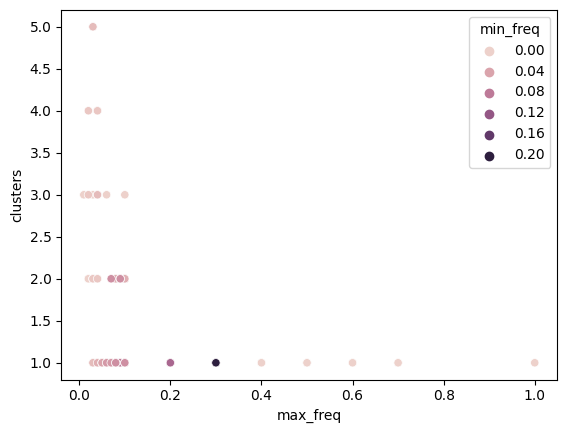
\includegraphics{figures/clusters_per_freq.png}

As for the rest of values of the table, they follow along with the explanation of the previous paragraph: a higher number of clusters implies more iterations to compute them, which requires more time to execute. The results obtained for the set of 250 words presents a similar trend, just with higher cost times. In this latter case, the reduction in the number of words from the 250 threshold is even more noticeable when the frequencies are very close.

As for a final set of "ideal" values, we have selected - and -, as they represent a middle point in between low values (which would result in more clusters but some unexpected behavior) and high values (stable behavior but very similar words).

\subsection{Mappers and reducers}

By default, the given script is executed using two mappers and two reducers, which, a priori, seems inefficient, as a higher number of processes would complete the execution faster. In order to test this hypothesis, we altered the \textit{ncores} flag, using values from 1 to 7 and check how this variation impacted the execution time, doing so for the two word sets generated beforehand. The maximum number of iterations was fixed to 10, as well as the initial number of clusters. For each number of cores and for each vocabulary size 10 executions were triggered, summarizing the average results obtained in the following tables.

\begin{table}
\begin{tabular}{||c c c c c c||}
 \hline
 Num cores & First iteration & Total time & Avg time per iteration\\ [0.5ex]
 \hline\hline
 1 & 3.565 & 49.102 & 5.455 \\
 \hline
 2 & 2.407 & 31.236 & 3.470  \\
 \hline
 3 & 2.299 & 26.896 & 2.989 \\
 \hline
 4 & 2.229 & 24.834 & 2.760 \\
 \hline
 5 & 2.238 & 23.716 & 2.635 \\
 \hline
 6 & 2.231 & 23.113 & 2.568 \\
 \hline
 7 & 2.689 & 27.937 & 3.104 \\
 \hline
\end{tabular}
\caption{MapReduce behavior when changing the number of cores. Vocabulary size of 100}
\end{table}

\begin{table}
\begin{tabular}{||c c c c c c||}
 \hline
 Num cores & First iteration & Total time & Avg time per iteration\\ [0.5ex]
 \hline\hline
 1 & 4.429 & 148.248 & 16.472 \\
 \hline
 2 & 3.009 & 81.236 & 9.026  \\
 \hline
 3 & 2.714 & 60.836 & 6.759 \\
 \hline
 4 & 2.591 & 49.904 & 5.544 \\
 \hline
 5 & 2.515 & 43.991 & 4.887 \\
 \hline
 6 & 2.472 & 39.894 & 4.432 \\
 \hline
 7 & 2.990 & 50.240 & 5.582 \\
 \hline
\end{tabular}
\caption{MapReduce behavior when changing the number of cores. Vocabulary size of 250}
\end{table}

The first conclusion is that the size of the vocabulary used does impact the execution time. We can observe that the values of the second table are always higher than in the first one, which makes sense as the amount of words is more than doubled. On the other hand, it is clear to see that the more cores used, the lesser the time needed to execute the whole process. This is specially true when jumping from 1 to 2 cores, and from 2 to 3. From this point onward the difference is not that noticeable.

However, when the number of cores is 7, the time does increase once more. This signals that using more cores is not always the best solution. This might seem counter-intuitive, as the more cores used, the more the work should be distributed and the faster the algorithm should execute. However, we need to take into account that there is an additional cost to using more cores, which is the overhead required to coordinate and synchronize all the processes. Given the results obtained, it would seem that for both vocabulary sized the optimal value is 6 cores, as with 7 cores the result gets worse and, presumably, increasing the value even more would result in even worse results.

As a final note, the first iteration is always considerably quicker than the others. This is due to the fact that on the first iteration the clusters are "stored" in a single document file each, so the operations needed to calculate the centroids are more immediate and quicker. For the other iterations, the centroid needs to be calculated through the documents assigned to each cluster, which implies a longer list of words to go through, which considerably increases the time needed to calculate the similarity.


\subsection{Most frequent words}

